\documentclass{sigcomm-alternate}

\begin{document}

\title{Net Neutrality, Bandwidth Usage and Government Regulations}
	
\numberofauthors{3}

\author{
	% 1st. author
	\alignauthor
	Raz Friman\\
	\affaddr{Southern Methodist Univeristy}\\
	\affaddr{5600 SMU Blvd. APT 1516}\\
	\affaddr{Dallas, Texas, 75206}\\
	\email{rfriman@smu.edu}
	% 2nd. author
	\alignauthor
	Jarret Shook\\
	\affaddr{Southern Methodist Univeristy}\\
	\affaddr{5555 Amesbury Dr. APT 1303}\\
	\affaddr{Dallas, Texas, 75206}\\
	\email{jshook@smu.edu}
	% 3rd. author
	\alignauthor Elena Villamil\\
	\affaddr{Southern Methodist Univeristy}\\
	\affaddr{5555 Amesbury Dr. APT 1303}\\
	\affaddr{Dallas, Texas, 75206}\\
	\email{mvillamilrod@smu.edu}
	\and  % use '\and' if you need 'another row' of author names	
	% 4th. author
	\alignauthor Jeffrey Artigues\\
	\affaddr{Southern Mehthodist University}\\
	\affaddr{9520 Amberton Pkwy.}\\
	\affaddr{Dallas, Texas, 75243}\\
	\email{jartigues@smu.edu}
}

\maketitle

\begin{abstract}
This paper will focus on the impact of laws enforcing Net Neutrality and the regulation of the Internet as a utility. Net Neutrality is a widely debated technical topic that is being discussed politically, as its implementation affects a significant range of individuals and companies.  The political discussions broaden the topic to focus on more than just the technical aspects, specifically the impacts net neutrality would have on the economic, political and business environments. In this paper, we will explore how bandwidth usage is affected by Net Neutrality, how prioritization can affect the network, how other countries which have implemented Net Neutrality compare to the US, and the economic and business implications of Net Neutrality. CONCLUSIONS GO HERE.
\end{abstract}



\section{Introduction}
In February 2014, Netflix issued a class action lawsuit against Comcast stating it was illegal for Comcast to throttle back Netflix speeds due to bandwidth usage.  The lawsuit ended with Netflix settling out of court with Comcast. This lawsuit proved that there is currently no net neutrality in the United States. This was a big motivation for reviewing regulations on Internet, not just in the US but also in Europe. Additionally, Japan has already implemented regulations in order to preserve Net Neutrality. Furthermore, two of the main foci of the latest bill passed by the FCC are to establish Net Neutrality and to regulate the Internet as utility. [Problem Statement]The question is how do these laws, in particular regulating the Internet as a utility, politically and economically affect the country, and how they affect the quality of service of Internet. 

[Basic Approach]
First, we define Net Neutrality as: “the principle according to which all Internet traffic is treated equally, without discrimination, restriction or interference, independently of its sender, recipient, type, content, device, service or application” \cite{gigaom}. In our research we start by analyzing current network traffic and draw conclusions on how net neutrality would affect this usage. Network traffic is significantly increasing, and in particular video streaming is the service increasing the most rapidly[Reference]. As of today, with the way Internet is being regulated this bandwidth usage is not a problem; however, if we add in the idea of net neutrality and add stricter limitations to what ISPs can do, then the quality of service may suffer.  For example, think of networking as a system of highways. If we allow all packets to travel in the same way without traffic enforcement (throttling), could we lose performance over the network as a whole? \cite{tandlInfographic}

Next, we examined the new bill passed by the FCC to regulate the Internet under net neutrality as a utility. This is a big change in several different aspects. First, it has economical effects for the ISPs, the consumers, and the government. For example, ISPs like Comcast and Verizon will lose the money from any agreement they had with companies like Netflix.  Thus they may increase increase their prices to compensate which will adversely affect the consumer. Not to mention, taxes may also increase the amount the end user will have to pay for Internet services. Two, it may affect the performance (quality of service) of Internet; e.g. is Internet speed going to be slower because ISPs will not be able to regulate the traffic the same way anymore. Third, it has political effects; for instance, how do this regulations affect taxes and government control over Internet which has not been regulated before. Lastly, we worked on comparing and finding relations between the bill passed in the US and the way Net Neutrality is working and it is being implement in Europe and Japan.

We start with an analysis of the current bandwidth usage. Then we expose an overview of the current bill passed by the FCC. In a later section we will discuss its different political, economical and technical implications. Afterwards, we talk about Net Neutrality in Japan and Europe and related to the US.


\section{Related Work}
There is an ever-growing collection of publications, articles, and news reports about Net Neutrality. Unfortunately, almost all of these sources usually include some degree of bias in them. In order to get unbiased information about this topic, we have to analyze multiple sources with all levels of bias from each side and combine their factual information together to get a better understanding of Net Neutrality. This includes reading White Papers published by major ISPs in addition to the articles published by the FCC favoring their Net Neutrality proposal. By combining these two heavily biased sources, we can extract the actual relevant information and create a view that is not biased towards any one side. 

[TALK ABOUT FCC OPINION HERE]Tom Wheeler, chairman of the F.C.C., has come out as a huge proponent of Net Neutrality \cite{FCCTomWheeler}. This will be shown later in the paper once we discuss this topic in more detail.


[TALK ABOUT ISPs OPINION HERE]
blah blah blah blah blah blah blah blah blah blah blah blah blah blah blah blah blah blah blah blah blah blah blah blah

We also reviewed the laws and regulations in effect in Europe and Japan where Net Neutrality is already established. In the next section, we compare these regulations with the new regulation passed in the United States and analyze how they relate and how they differ.

\section{Research Approach}

\subsection{Bandwidth Usage}
As we transition into an even more interconnected world with the Internet of Things, real time information most likely in small quantities is expected to be in high demand and readily available. Streaming services like Netflix still continues to dominate the global amount of network traffic[Source]. usage on the Internet is constantly evolving, and the infrastructure supporting the Internet needs to be able to adapt to these changes. According to Cisco’s annual VNI report, video streaming currently accounts for over 60\% of traffic usage on the Internet \cite{cisco}. Using current projections and traffic analysis, they predict that within 5 years, video streaming will grow to account for over 80\% of traffic usage. This is a huge amount of data that must seamlessly be transported across the world. If the current infrastructure is not set up and managed correctly, there will be drastic consequences. One issue regarding how ISPs handle this massive growth in demand has already occurred, and the solution was not very elegant.

Between 2013 and 2014, before any FCC proposals of Net Neutrality were introduced, Netflix and Comcast got into an argument over bandwidth usage. Netflix, with its increasing growth, was taking up more and more of the bandwidth from its ISPs. When an ISP’s bandwidth is filled with many packets of Netflix streaming, there is less room to transmit other types of traffic. In order to remediate this issue, Comcast demanded a fee from Netflix for using up a majority of its bandwidth. At the same time, it used this excuse to begin throttling back Netflix traffic in order to allow more room for other types of traffic. Netflix stated that this sort of action was unfair and against the basic principles of Net Neutrality. Therefore, they went to court to solve their issues. As the court proceedings continued, Comcast continued to throttle back Netflix’s bandwidth speed further and further. Eventually, in February of 2014, Netflix and Comcast settled out of court and Netflix paid Comcast an undisclosed amount under a peering agreement. As soon as this agreement was reached, Netflix’s speed on Comcast’s network went up over 45\% within 2 months. Afterwards, Verizon took advantage of this situation by demanding a premium from Netflix as well. As Netflix’s customers complained about slowing speeds, Netflix had no choice but to pay the fee in order to restore its customers expected quality of service. The bandwidth speeds for Netflix on both Comcast and Verizon can be seen on Figure \ref{fig:netflix} below. Figure ~\ref{fig:netflix} demonstrates that as soon as an agreement was made, the bandwidth throttling immediately ceased and return to normal speeds.

These actions demonstrate a flaw in fair competition that Net Neutrality has the potential to fix. If these negotiations and agreements continue to form, ISPs like Comcast and Verizon will be able to charge both the customers and content providers for using bandwidth. Additionally, this will give larger companies an unfair advantage in gaining more access to bandwidth as compared to small business and startups. A system that supports large corporations and makes competition with smaller businesses impossible is harmful to consumers and creates a large barrier of entry for all Internet-related businesses.



\begin{figure}
	\label{fig:netflix}
	\hspace*{-0cm}
	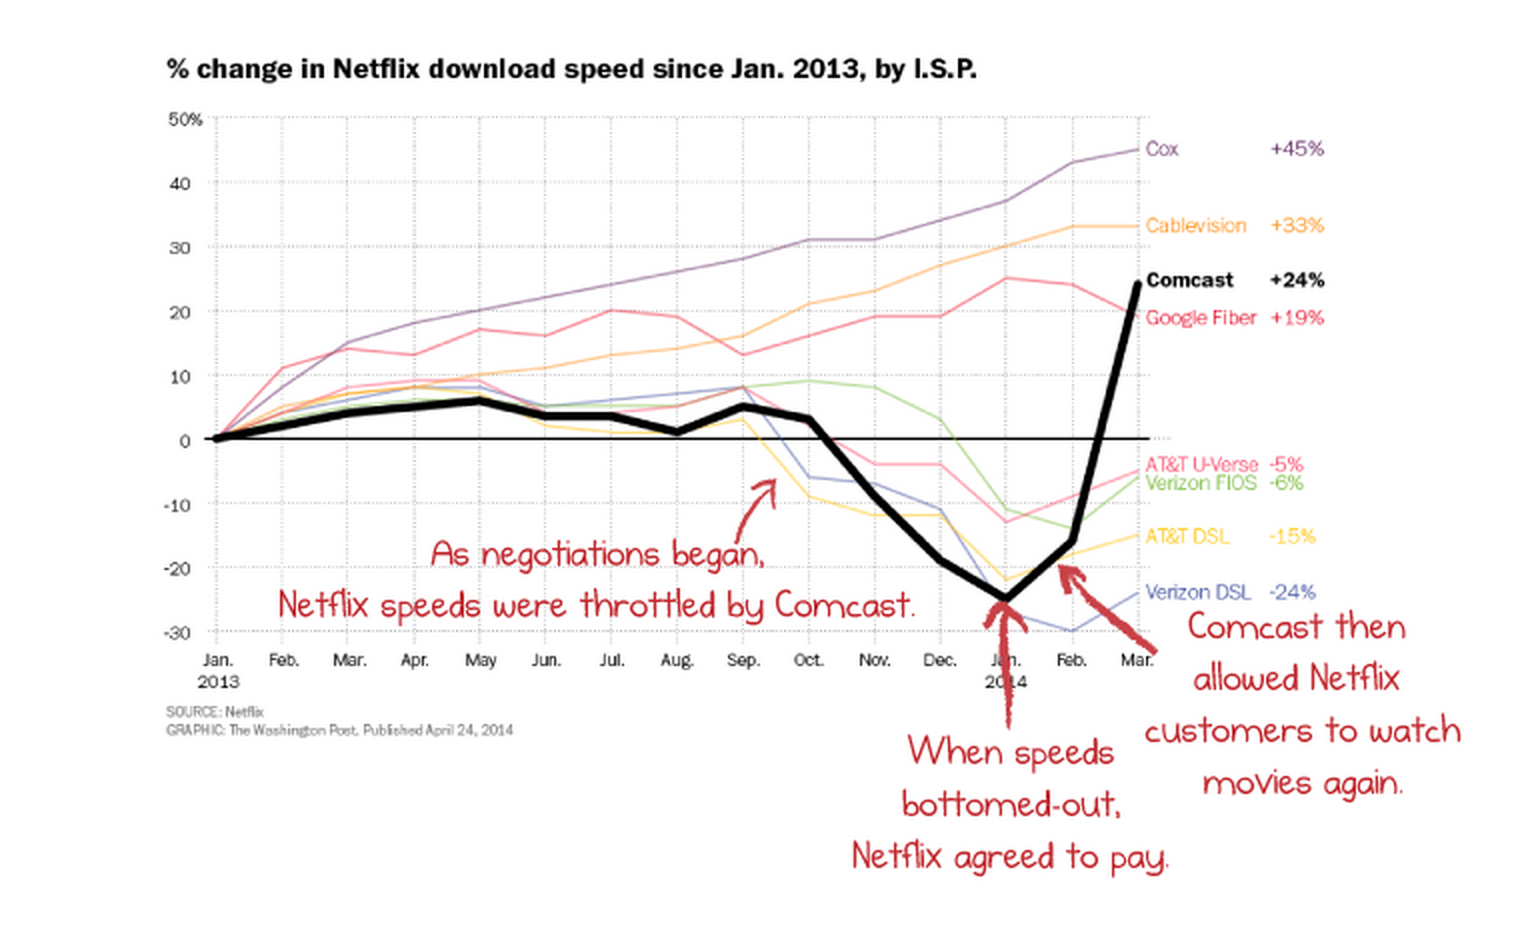
\includegraphics[scale=.20]{NetflixGraph.png}
	\caption{Graph comparing Netflix bandwidth speeds over time from different ISPs.}
\end{figure}

%\begin{figure}
%	\centering
%	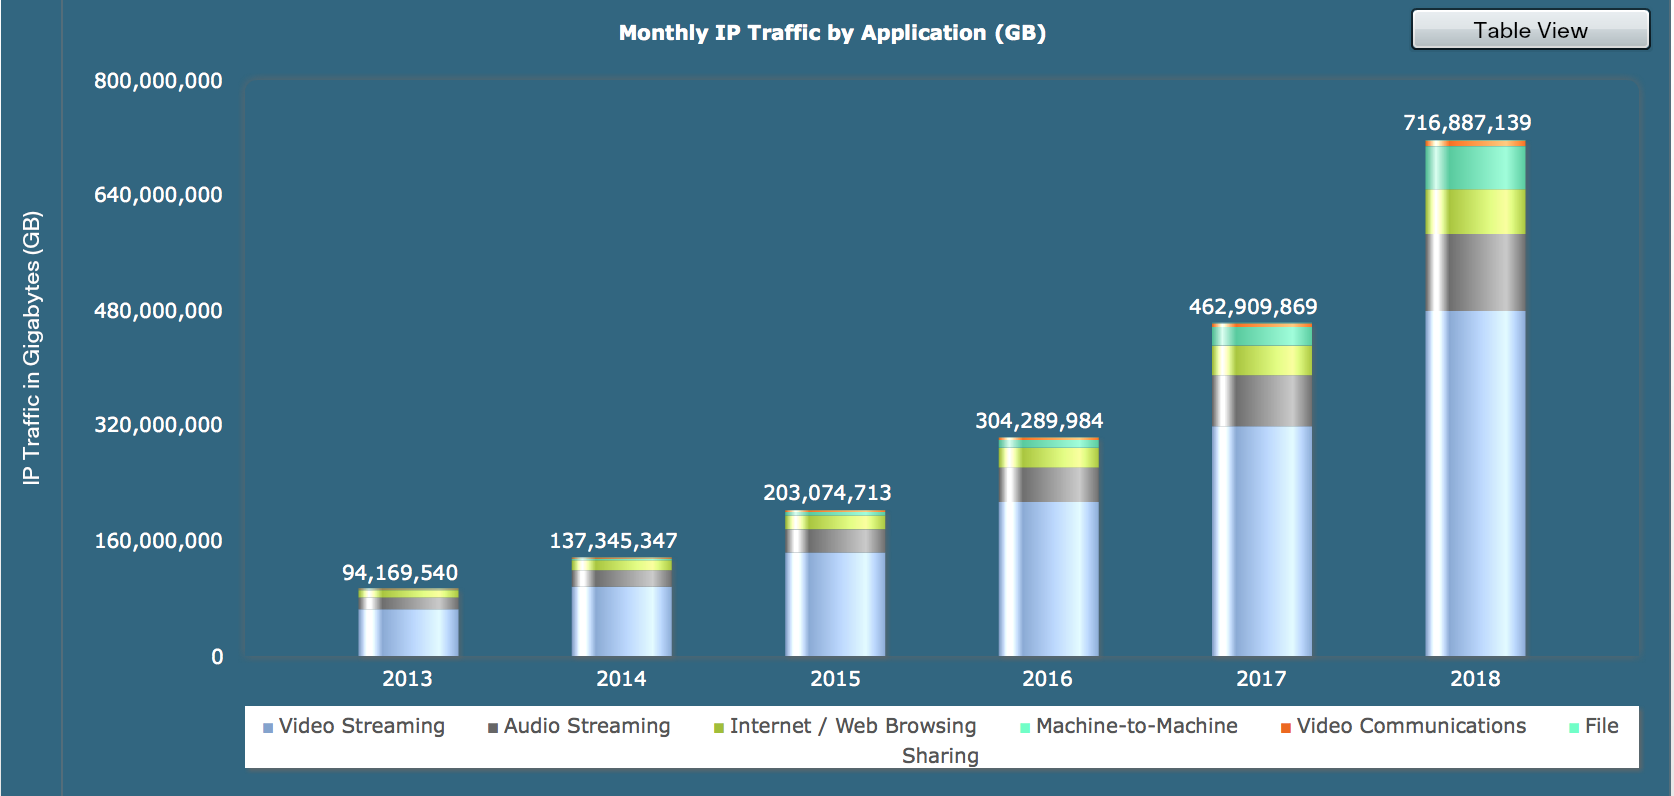
\includegraphics[scale=.29]{BandwidthGraph.png}
%	\caption{Graph comparing Netflix bandwidth speeds over time from different ISPs.}
%end{figure}




\subsection{Net Neutrality in Europe}

In September of 2013, the European Commission (EC) proposed the European Union’s new package of telecom laws. This package included the Net Neutrality legislation. With this legislation the EC aimed to protected Net Neutrality in the European Union (EU) and to stop blocking or throttling of competing data. However, this legislation also gives ISPs freedom to higher speeds or quality to specialized services as long as the standard Internet is not harmed from it \cite{economics}.

In April of 2014 the European Parliament voted and passed the telecom law reform proposed by the EC. They did add some amendments to properly define and protect Net Neutrality. Two amendments worth notice are 235 and 236. Amendment 235 gives a strong definition of “specialized services”; the goal of this amendment is give ISPs string constraints to what they can consider outside standard Internet. Amendment 236 specifies that this specialized services shall only be provided if the network has capacity enough to support standard services plus the specialized services without any detrimental result on the quality of Internet. In addition this amendment also determinants that providers cannot discriminate between equivalent services and applications \cite{gigaom}.

This reforms happen close after the Netflix deal with Comcast and Verizon were approved in United States. In particular, The fact that amendment 235 gives a strong definition of “specialised services” will keep ISPs from putting into this category services that do not belong there, such as Netflix, in order to get extra money from them.

David Meyer, European correspondent for tech site Gigaom, has an interesting opinion on the new regulation and on Net Neutrality in Europe versus United States. According to him, the new laws will allow consumers to be in control. He also claims that ISPs will not be able to higher the costs because of the existence of a high competitive mark, meaning if ISPs dramatically increase their prices then they will lose customers*. Moreover, he also gives his opinion on Net Neutrality in the EU versus Net Neutrality in US. According to him in the US ISPs can degraded services that do not match their interests, and this is not the interest of the consumer. He also affirms that in the US new entrants to the market can be disadvantaged because they do not have enough money to pay ISPs\footnote{Meyer refers this part specifically to UK, but it can be applied to Europe in general.  At the same time it gives ISPs the alternative to refuse or get extra money for supporting services that because of their specific necessities will in fact be outside the standard.} \cite{inthenews}.


In conclusion, the EU has Internet regulations that enforce net neutrality, and that restrict ISPs range of action. However, none of this regulations mention regulating Internet as a utility. It is not fair to straight out compare the EU with US since there a lot of different characteristics that makes them unique. However, the fact that Europe is working under net neutrality laws without utility or pricing regulations, and that the ISPs in Europe have no problems proving consumers with good quality  is a very important fact to take into account.



\subsection{Net Neutrality in Japan}

Japan in comparison to the EU, has had Net Neutrality for a longer period of time.  They make a good case study to how effectively their country has been able to handle bandwidth congestion.  Most importantly, Japan differs from the United States in that there is more ISP competition.  This is guaranteed by regulations from the government, there are certain companies which are unable to grow past the point they are.

As previously explained, if there ever is a situation where 100\% of a network is used, all packets being sent past that point are dropped.  People would experience loss of service, dramatic slowdowns and general unusability.  Because all Internet traffic must be treated equally in a Net Neutral environment, there is no way to individually contain users who may be using the largest portion of traffic.  For example, if there ever was a case in which a company was using 80\% of the network, it makes little sense to throttle back every user of that network when the majority of the network could be unaffected by throttling that one company.  With that said, this is not possible under Net Neutrality laws, as you would not be giving equal treatment to everyone on the network, one or two may be singled out and contained.

Japan, addressing this problem has set a few different things into place.  First, the country has never experienced a “blackout” or reached 100\% network usage.  Therefore, so far their strategy has been successful.  However, they have come close, specifically in 2007 90\% of the entire Japanese download bandwidth was used, with 80\% of its upload bandwidth being used during peak hours.  

\subsection{Economic and Business Implications}

Innovation

Feasibility

Economic/Infrastructure

Network efficiency


\bibliographystyle{unsrt}
\bibliography{bib}

\end{document}
